\section{Parametrized Neural Network}
\subsection{Discriminating Masses}
When introducing the \ac{PNN} in section \ref{subsec:PNN}, I mentioned that by including the masses of the introduced particles
in the feature set, we motivate and individualistic tuning for each mass combination in the signal set. To test if this is indeed what 
happens, I will in this section present results where I manually assign different mass combinations the same label. The hope 
is that if indeed the \ac{PNN} has been able to tune individually for each mass combination, then the \ac{PNN} should perform best 
when the events are correctly labeled compared to when they are not. 
\\
In figure \ref{fig:PNN50250Dist} I have drawn the distribution of the output from the trained \ac{PNN} architecture 
(see section \ref{subsec:PNNArch}). The model was trained using the \ac{FSMLM} data set. In figure \ref{fig:PNN50250Dist},
4 signals have been included; ($\tilde{\chi}_1=50$, $\tilde{\chi}_2=250$GeV), ($\tilde{\chi}_1=100$, $\tilde{\chi}_2=200$GeV), 
($\tilde{\chi}_1=200$, $\tilde{\chi}_2=300$GeV) and ($\tilde{\chi}_1=150$, $\tilde{\chi}_2=250$GeV). All data, including 
both signal and background were given the labels of $50$ and $250$. In figure \ref{fig:PNN50250Dist} the full output range
is included, whereas in figure \ref{fig:PNN50250Dist_95} only the output in the range $0.975-1$ has been included. From studying  
the figures and the corresponding legends, we can deduce that the signal which is given the correct label is also the signal which 
has the highest percentage of conserved events when applying a simple cut off $0.975$\footnote{This is further evident when studying 
the efficiency rates in table \ref{table:PNNSigComp}.}.\\
\begin{figure}
    \makebox[0.95\linewidth][c]{%
    \centering
    \begin{subfigure}{.5\textwidth}
        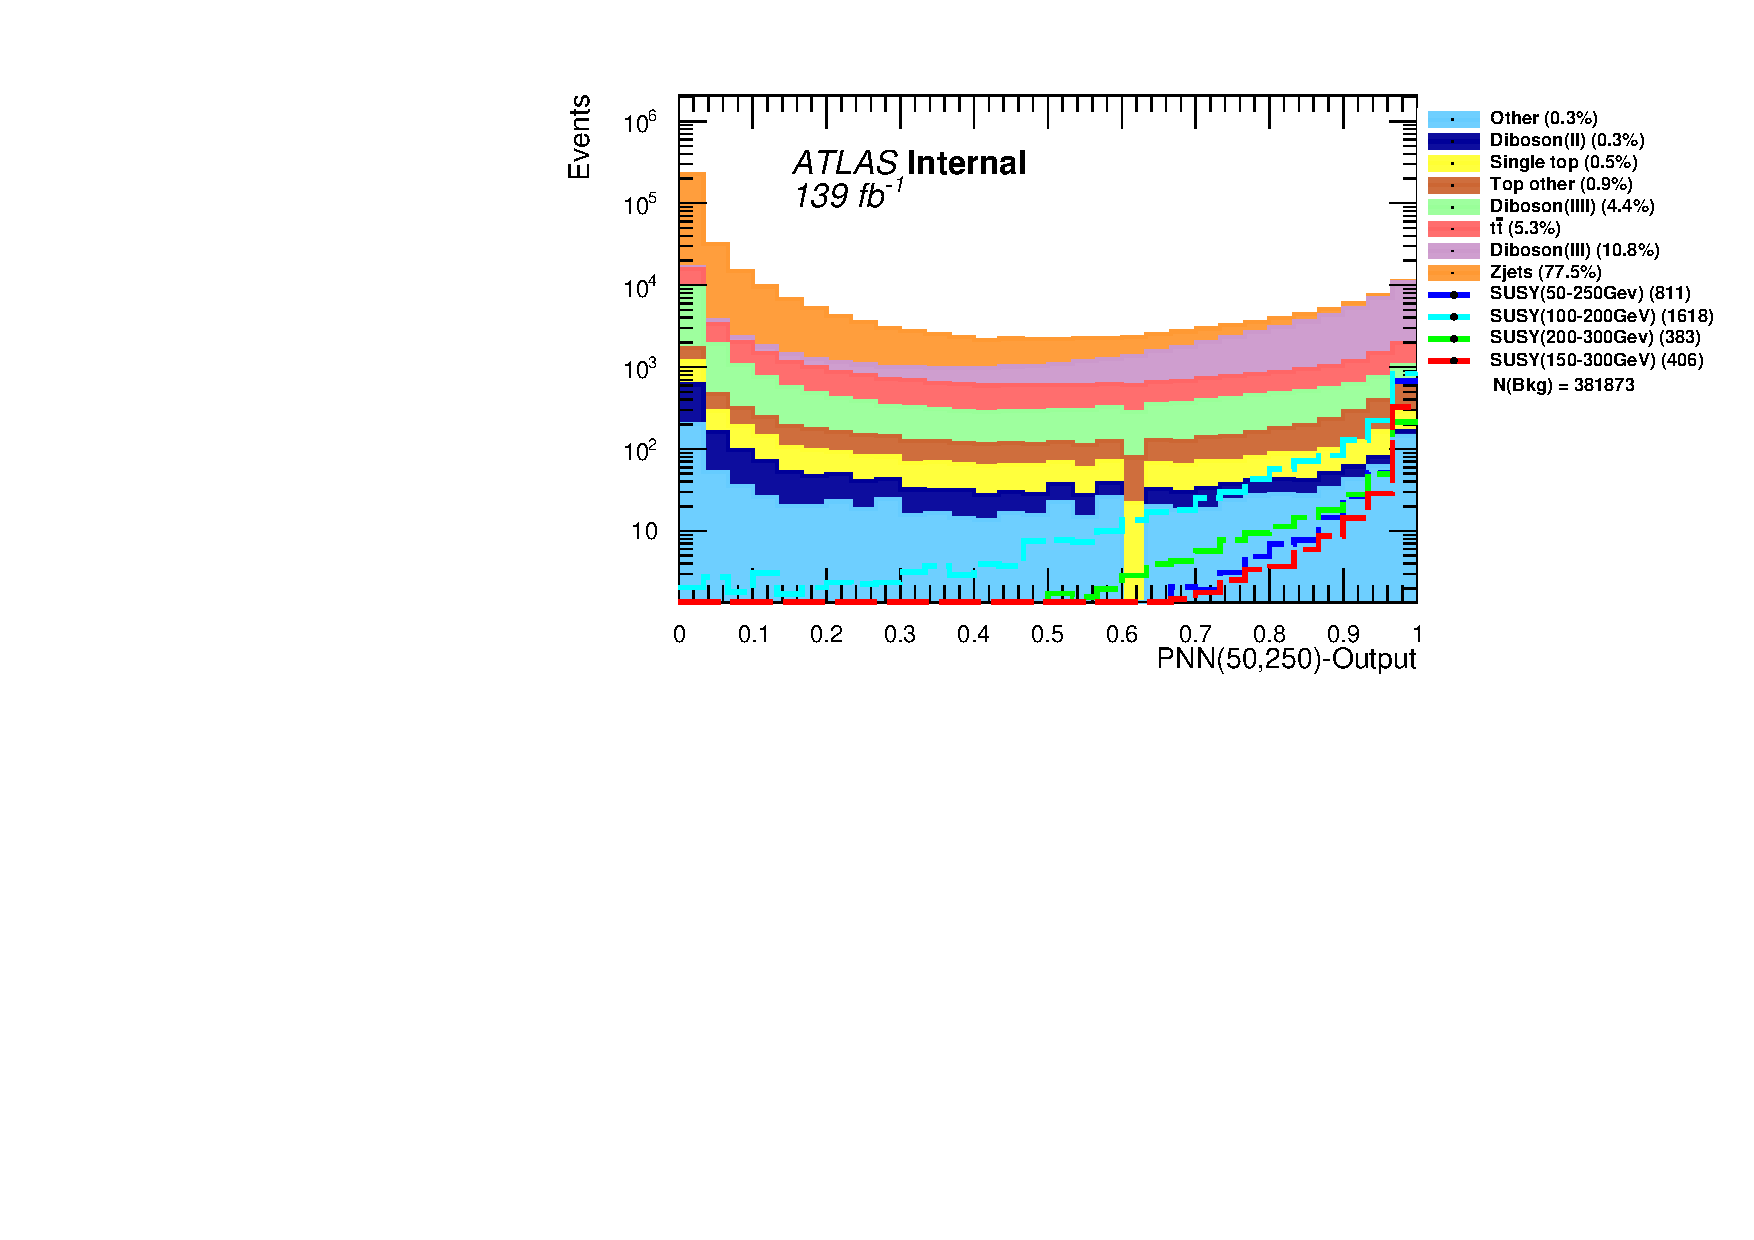
\includegraphics[width=\textwidth]{Figures/MLResults/NN/SUSY/MLDist/PNNDistTest/PNN50250Dist.pdf}
        \caption{}
        \label{fig:PNN50250Dist}
    \end{subfigure}
    \hfill
    \begin{subfigure}{.5\textwidth}
        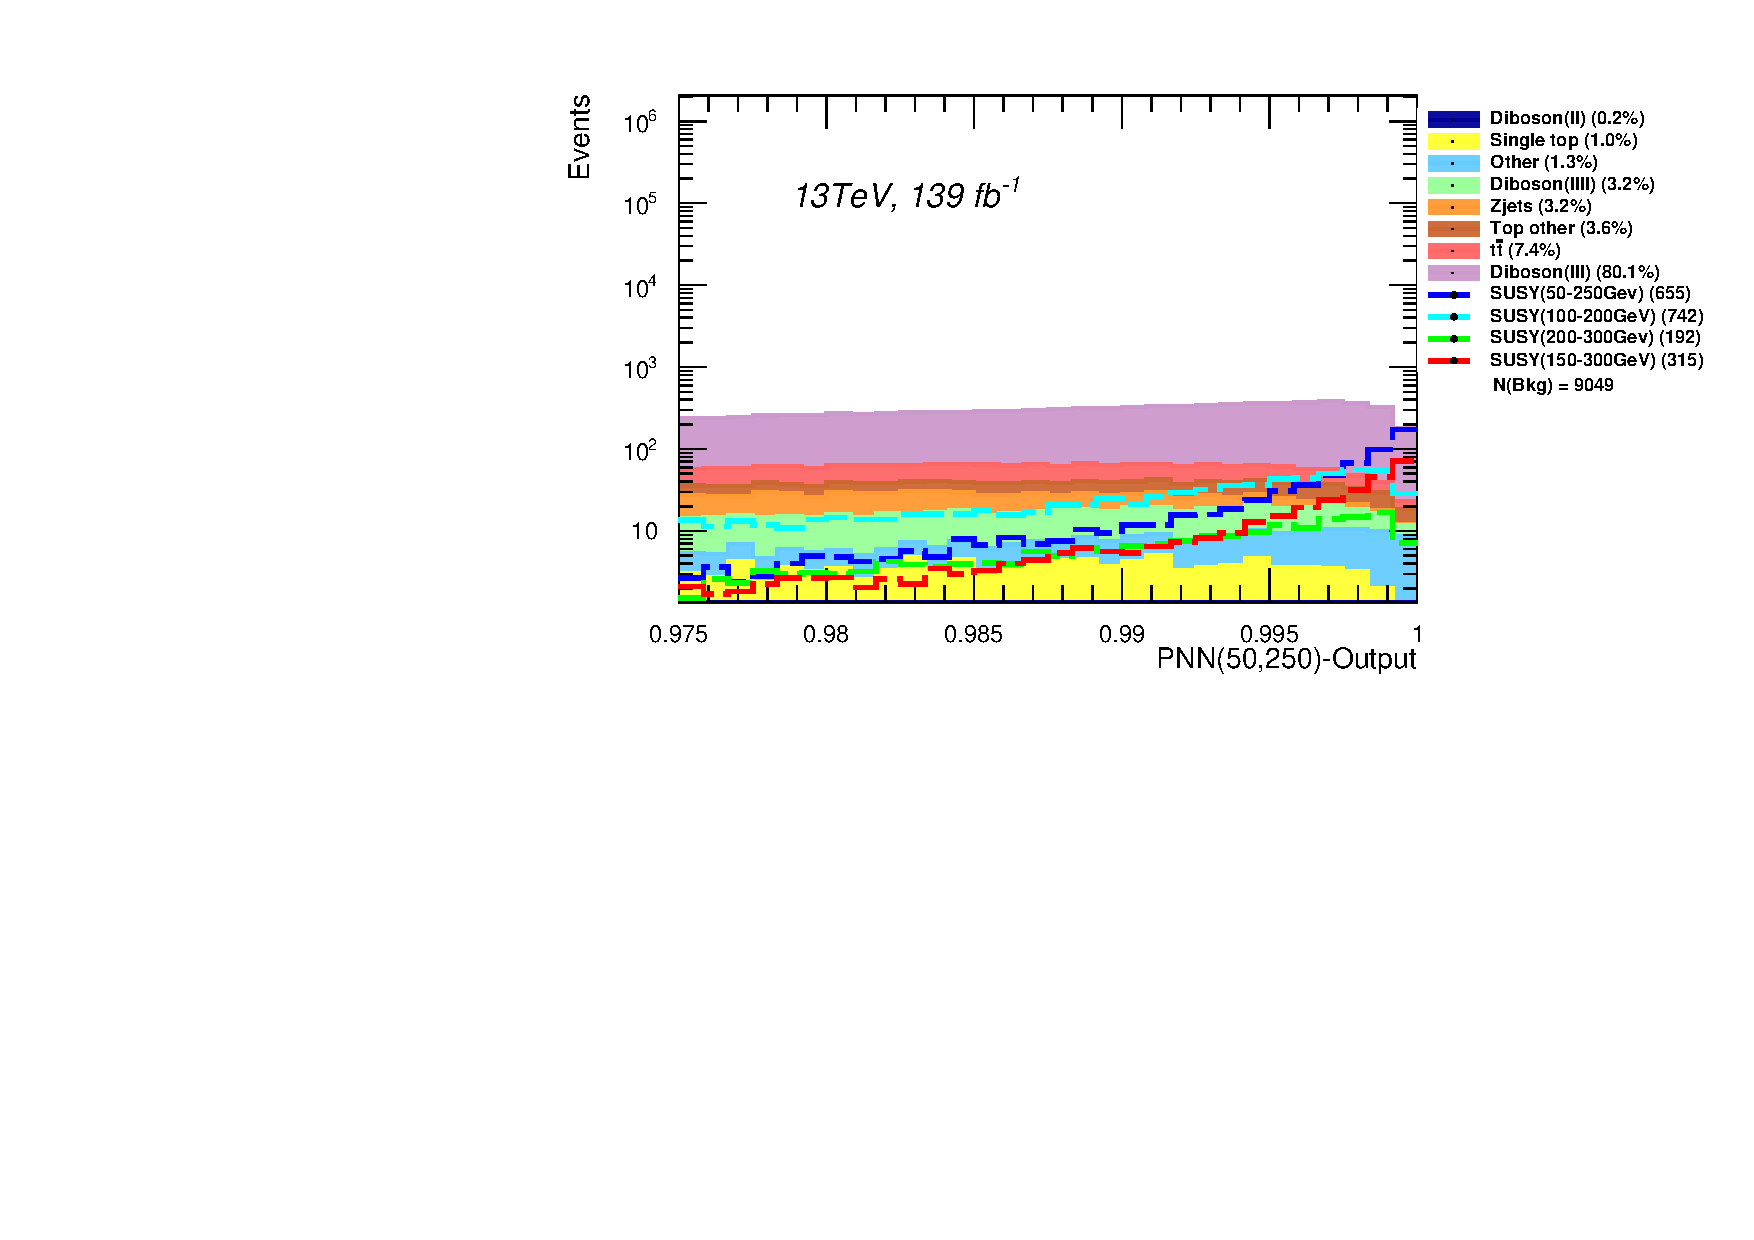
\includegraphics[width=\textwidth]{Figures/MLResults/NN/SUSY/MLDist/PNNDistTest/PNN50250Dist_C7.pdf}
        \caption{}
        \label{fig:PNN50250Dist_95}
    \end{subfigure}
    }
    \caption{The output distribution from a trained \ac{PNN} model for the background and signals with 4 different mass combinations:
    ($\tilde{\chi}_1=50$, $\tilde{\chi}_2=250$GeV), ($\tilde{\chi}_1=100$, $\tilde{\chi}_2=200$GeV), 
    ($\tilde{\chi}_1=200$, $\tilde{\chi}_2=300$GeV) and ($\tilde{\chi}_1=150$, $\tilde{\chi}_2=250$GeV), and where all the data were given the 
    parameter features of ($\tilde{\chi}_1=50$, $\tilde{\chi}_2=250$GeV). The figure includes the full output range (\ref{fig:PNN50250Dist}) 
    and the output ranging from 0.975-1.00 (\ref{fig:PNN50250Dist_95}).}
    \label{fig:PNN50250}
\end{figure}
In section \ref{sec:XGBoost} I presented results indicating that some signals were easier to separate from background than others. This leads me to the 
question; did the \ac{PNN} perform better on the signal with ($\tilde{\chi}_1=50$, $\tilde{\chi}_2=250$GeV) because of the labeling, or simply
because this particular signal was easier to separate. To answer this question I conducted a second test. In figure \ref{fig:PNN200300DistComp} 
I repeated the analysis described in the paragraphs above, but where all the signals were given the label ($\tilde{\chi}_1=200$, $\tilde{\chi}_2=300$GeV).
Similarly to the previous results, I drew the output for the full output range (\ref{fig:PNN200300Dist}) and after a cutoff off $0.975$ (\ref{fig:PNN50250Dist_95}).
Via the examination of the two figures, we can indeed see that my assumption was right. By giving events with ($\tilde{\chi}_1=50$, $\tilde{\chi}_2=250$GeV) the 
wrong label, the \ac{PNN} still achieved the highest performance when predicting on said mass combination.\\
\begin{figure}
    \makebox[0.95\linewidth][c]{%
    \centering
    \begin{subfigure}{.5\textwidth}
        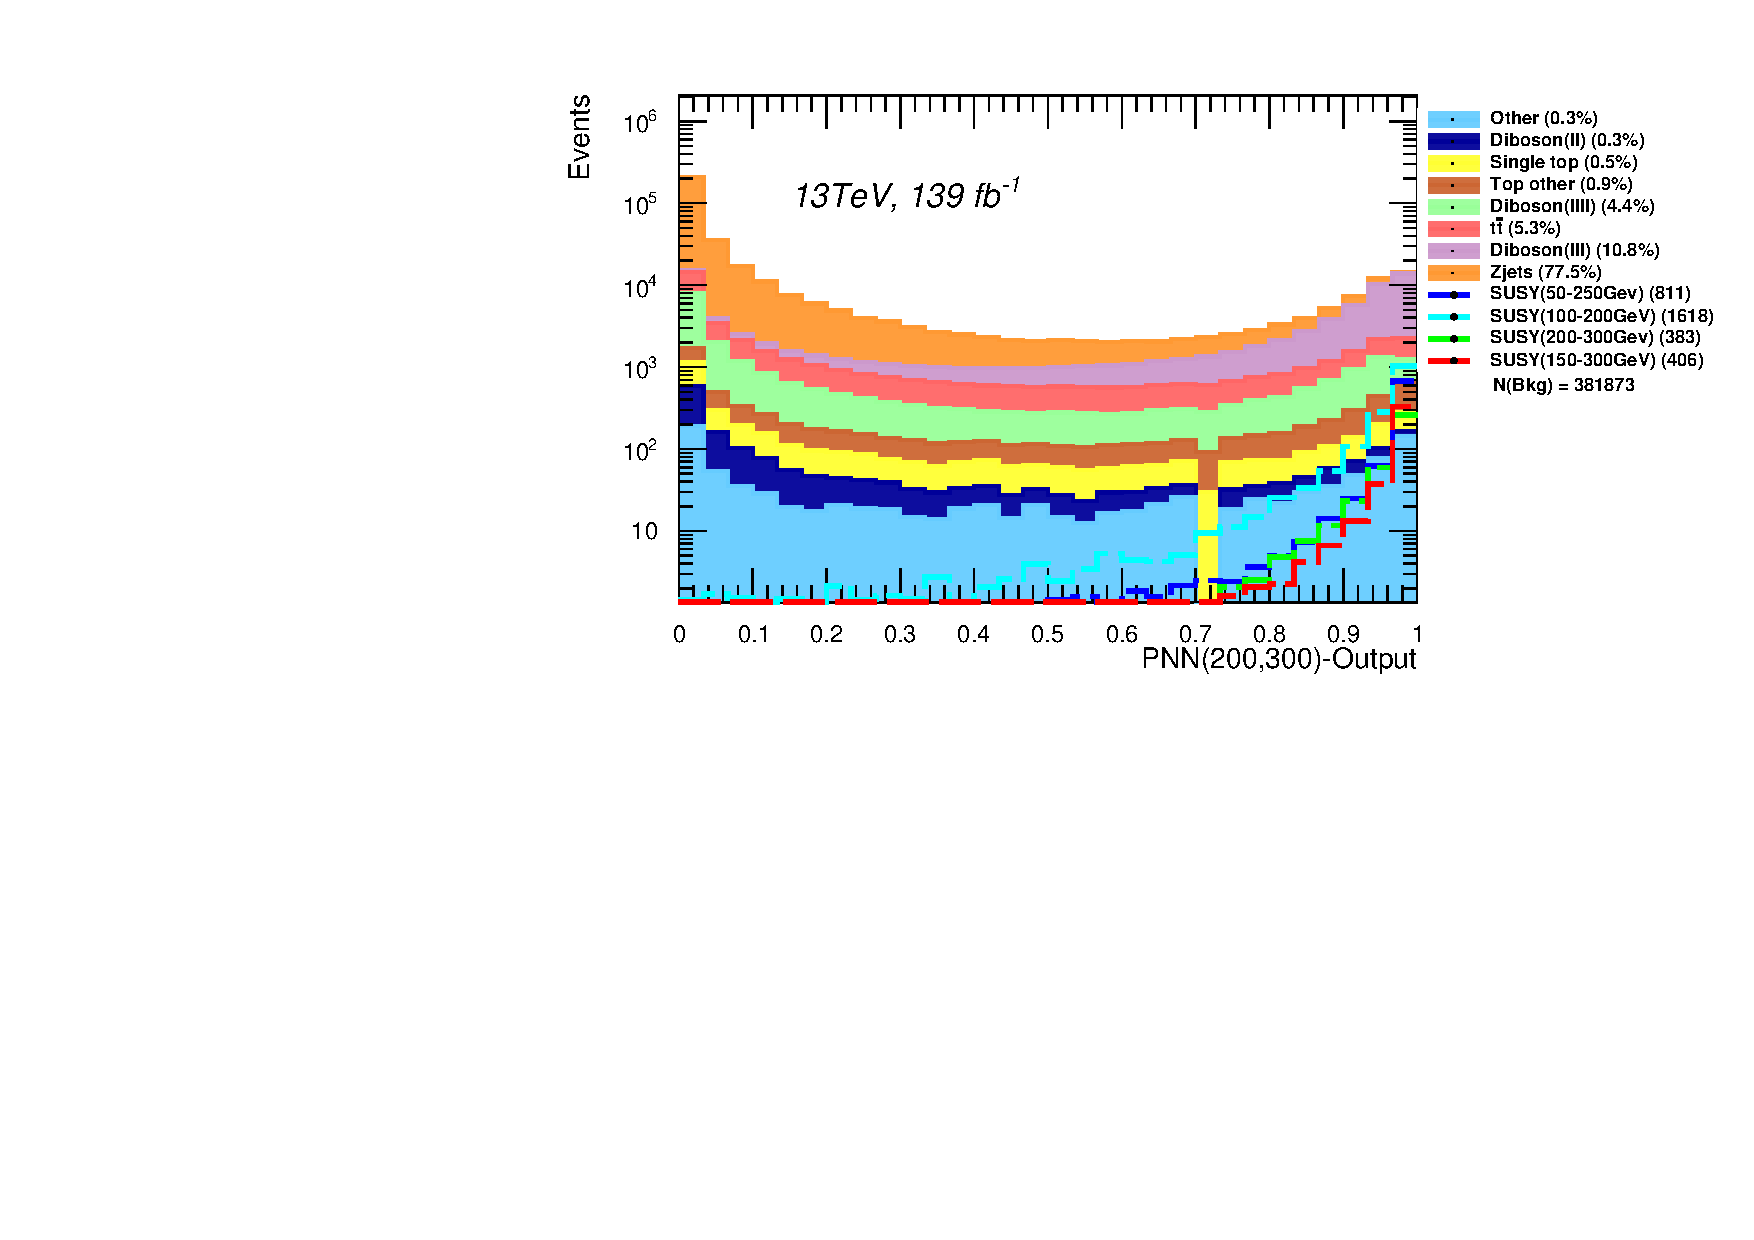
\includegraphics[width=\textwidth]{Figures/MLResults/NN/SUSY/MLDist/PNNDistTest/PNN200300Dist.pdf}
        \caption{}
        \label{fig:PNN200300Dist}
    \end{subfigure}
    \hfill
    \begin{subfigure}{.5\textwidth}
        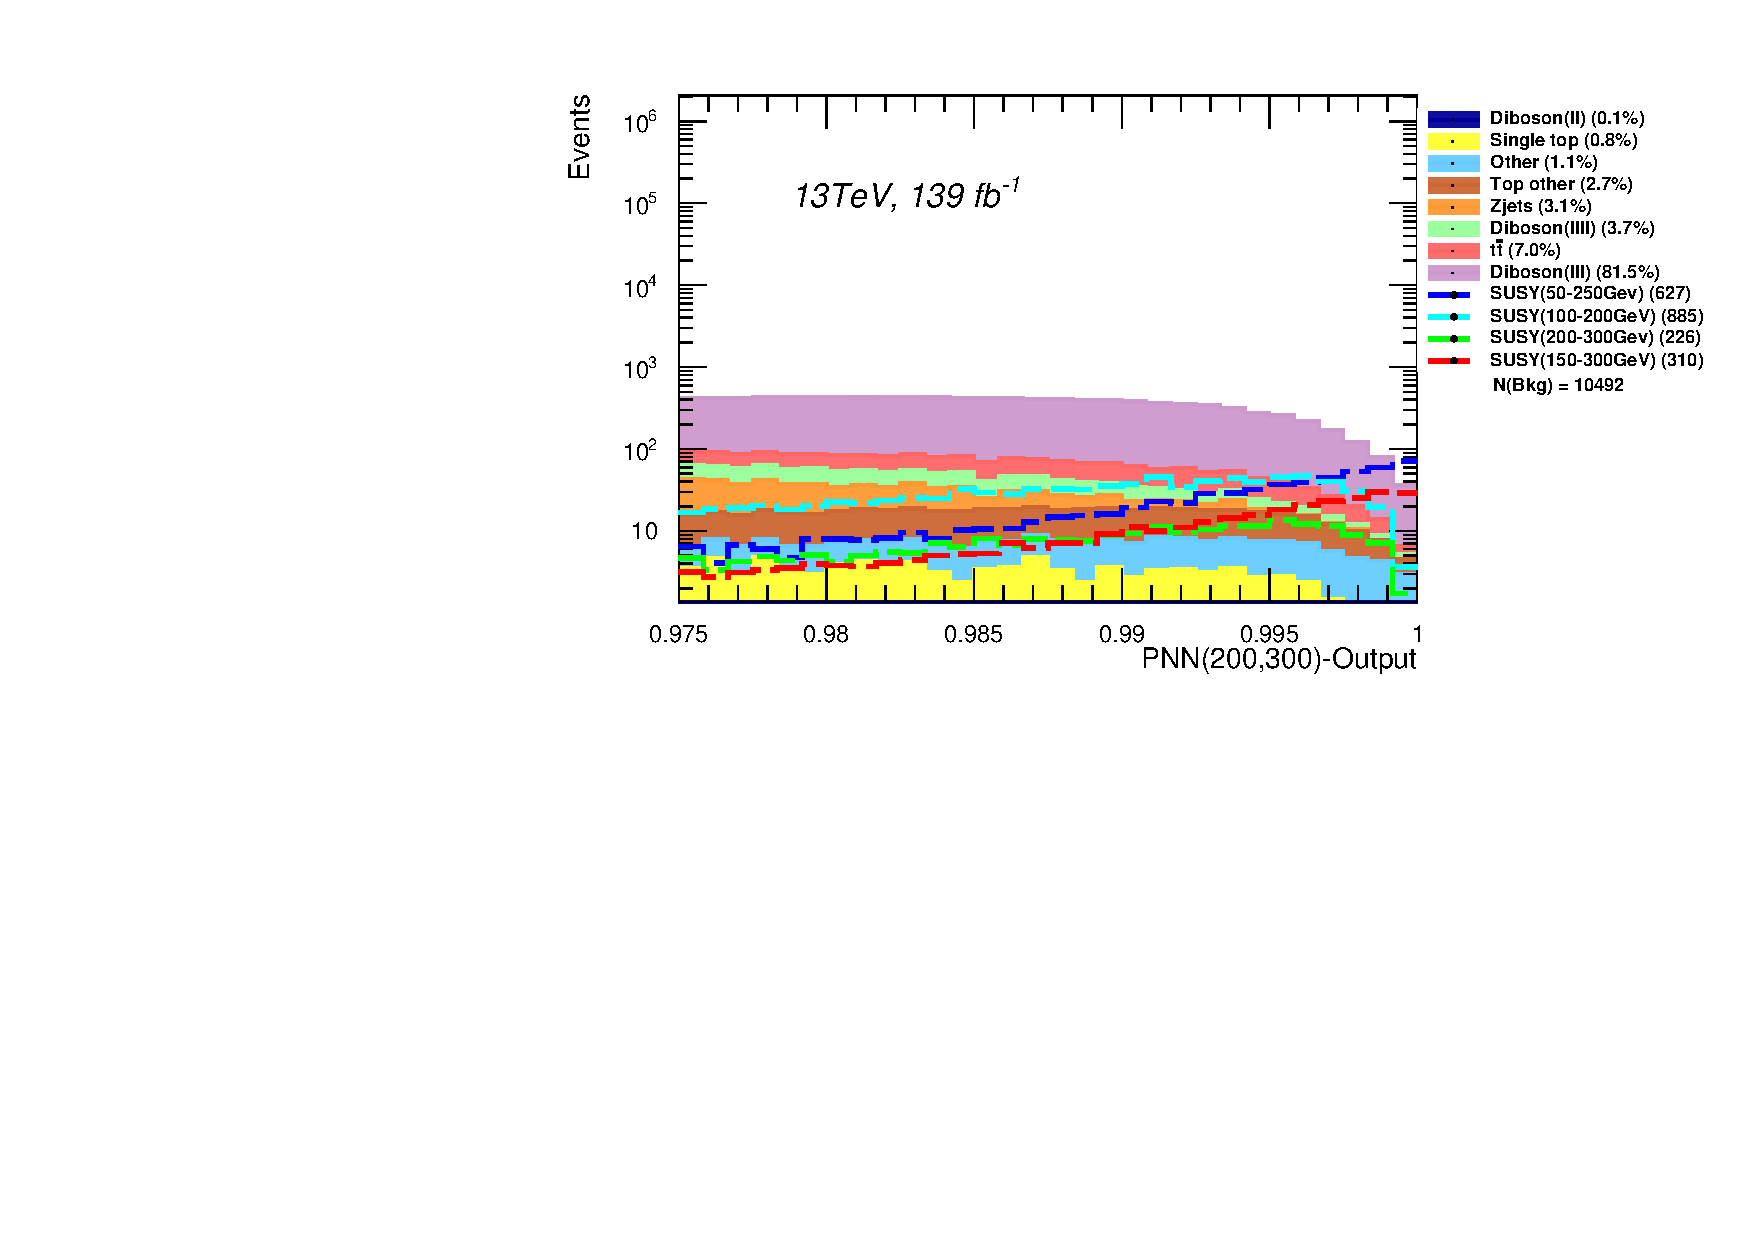
\includegraphics[width=\textwidth]{Figures/MLResults/NN/SUSY/MLDist/PNNDistTest/PNN200300Dist_C7.pdf}
        \caption{}
        \label{fig:PNN200300Dist_95}
    \end{subfigure}
    }
    \caption{The output distribution from a trained \ac{PNN} model for the background and signals with 4 different mass combinations:
    ($\tilde{\chi}_1=50$, $\tilde{\chi}_2=250$GeV), ($\tilde{\chi}_1=100$, $\tilde{\chi}_2=200$GeV), 
    ($\tilde{\chi}_1=200$, $\tilde{\chi}_2=300$GeV) and ($\tilde{\chi}_1=150$, $\tilde{\chi}_2=250$GeV), and where all the data were given the 
    parameter features of ($\tilde{\chi}_1=200$, $\tilde{\chi}_2=300$GeV). The figure includes the full output range (\ref{fig:PNN50250Dist}) 
    and the output ranging from 0.975-1.00 (\ref{fig:PNN50250Dist_95}).}
    \label{fig:PNN200300DistComp}
\end{figure}
To further study this result, I created a table of the efficiencies of each mass combination after applying a simple cut of $0.975$. The results are represented in 
table \ref{table:PNNSigComp}. It is evident from table \ref{table:PNNSigComp} that the \ac{PNN} achieves the highest performance when events are given the correct label, 
although not by much. Another interesting observation is that events with ($\tilde{\chi}_1=100$, $\tilde{\chi}_2=200$GeV) seem to prefer the label of 
($\tilde{\chi}_1=200$, $\tilde{\chi}_2=300$GeV) over that of ($\tilde{\chi}_1=150$, $\tilde{\chi}_2=250$GeV), despite the latter mass combination being closer 
in mass. A possible explanation is that the difference in mass ($\Delta m = |m_{\tilde{\chi}_1} - m_{\tilde{\chi}_2}|$), influences the trends in the data, similarly 
to what we saw that size of mass does. Regardless, from \ref{table:PNNSigComp}, we can deduce that the \ac{PNN} does in fact discriminate between mass combinations 
and tune for them independently.
\begin{table}
    \centering
    $
    \begin{array}{ccccc}
        \hline \text { \backslashbox{\textbf{Label}}{\textbf{Channel}} }  & \text {$(50,250)$}& \text {$(100,200)$} & \text {$(150,300)$} & \text {$(200,300)$} \\
        \hline\text {$(50,250)$}   & \text { $\bf{80.8}\%$ } & \text { $45.8\%$ } & \text { $\bf{77.5}\%$ } & \text { $50.1\%$ } \\
        \hline\text {$(200,300)$}   & \text { $77.3\%$ } & \text { $\bf{54.6}\%$ } & \text { $76.3\%$ } & \text { $\bf{59.0}\%$ } \\
        \hline
    \end{array}
    $
    \caption{A listing of the remaining procentage of each mass combination in the output range 0.975-1.00 using the 
    labels ($\tilde{\chi}_1=50$, $\tilde{\chi}_2=250$GeV) and ($\tilde{\chi}_1=200$, $\tilde{\chi}_2=300$GeV) respectively.}
    \label{table:PNNSigComp}
\end{table}

\subsection{Sensitivity Result}
In this section I will present the achieved sensitivity by the \ac{PNN} on the original signal set. In figure \ref{fig:PNNGridSig}, I present a grid displaying the sensitivity 
of the \ac{PNN} on the original signal set. Similarly to the previous models', the figure indicates that the \ac{PNN} is able to achieve a much higher sensitivity on the lower
masses. The most notable difference to the previous models, is the range of significance. The \ac{PNN} almost doubles the highest significance achieved by any previous model
(from 2.44 to 4.14), and simultaneously achieves the lowest significance (now 0.30). The most probable explanation to this result is the 
distribution of parameters for the background. In section \ref{subsec:PNN}, I described how the background is randomly assigned parameters such that the 
percentage of background with a given label is equal to the percentage of the signal with said label. In other words, the higher the statistics for a given mass combination,
the higher the amount of background will be "linked" to it. Inn the same section I also described the hope that the parameters would shift the 
output from the initial layer in a way that motivates individualistic training. If this is true\footnote{For a network of this depth, it is very hard to explain what happens during training.
Lack of explainability is in fact one of the biggest downsides to deep networks.} it means that masses with larger statistics, are given larger amounts of background to train with. 
This could explain the uneven performance by the \ac{PNN}.
\begin{figure} 
    \makebox[\linewidth][c]{%
    \centering
    \begin{subfigure}{.65\textwidth}
        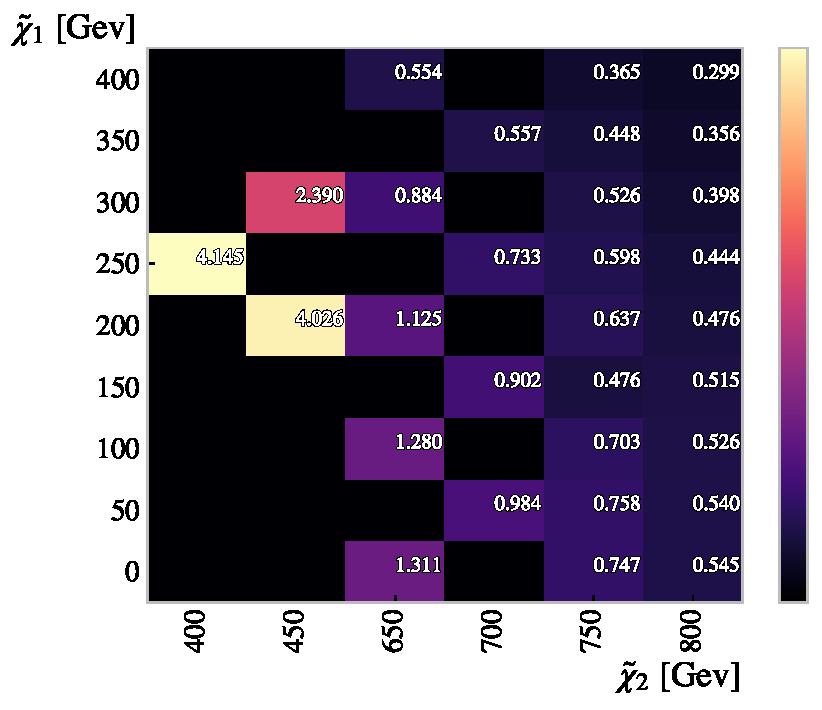
\includegraphics[width=\textwidth]{Figures/MLResults/NN/SUSY/Grid/PNNGridSig.pdf}
    \end{subfigure}
    }
    \caption{A grid displaying the achieved significance on the original signal set, using the signal region 
    created by the \ac{PNN} network.}
    \label{fig:PNNGridSig}
\end{figure}